\section{Fuzzing Run with AFL++}
\label{sec:fuzzrun}

SecureBank~PT exists only as a design, so the fuzzing tool was run on an
open-source project that can be built locally. The target is
cJSON~\cite{cjson}, a JSON parser written in ANSI~C as a single source
file of about 3{,}000 lines, used in embedded and IoT firmware. Every
SecureBank request is JSON, and vectors FZ-01 to FZ-03 aim at this kind
of parser. Two releases were fuzzed under the same conditions: 1.7.10,
from December 2018, and 1.7.19, the latest release, from September 2025.
Release 1.7.11 fixed out-of-bounds accesses in \texttt{cJSON\_Minify}
that were published as CVE-2019-11834 and
CVE-2019-11835~\cite{cve201911834}. The run therefore checks two things:
whether a short campaign finds faults that are known to exist, and
whether it reports anything on the fixed code.

\subsection{Setup and Steps}

The run used a laptop with an AMD Ryzen~7 5800H (16 threads) and 30~GB
of RAM, running Arch Linux with kernel 7.2 and clang 23.1.4.

\begin{enumerate}
\item AFL++ 5.04a~\cite{aflpp2020} was built from its stable branch
(commit \texttt{d798677}).
\item The harness is the one the project keeps for OSS-Fuzz,
\texttt{cjson\_read\_fuzzer.c}, linked with the AFL++ driver so that it
runs in persistent mode. Its first four bytes set four options (minify,
require termination, formatted and buffered printing), and the input
must end with a NUL byte. After a successful parse, it prints the tree
and, if minify is set, passes a copy of the input to
\texttt{cJSON\_Minify}.
\item Each release was compiled with \texttt{afl-clang-fast},
\ac{ASan} and \ac{UBSan}. A second build of each release, with the same
sanitizers and without AFL++ instrumentation, replays the crashes.
\item The 13 seeds are the 11 sample files of the project, converted to
the harness format, and two synthetic transfer orders in the shape of
the SecureBank \ac{API}. The dictionary is \texttt{json.dict} from the
project.
\item One \texttt{afl-fuzz} instance per release ran for 15~minutes, both
in parallel on separate cores.
\item Every saved crash and hang was replayed on both replay builds. The
inputs were grouped by root cause, and one input per group was minimised
with \texttt{afl-tmin}.
\end{enumerate}

The main commands for release 1.7.10 were the following; release 1.7.19
used the same commands with its own paths.

\noindent\begin{minipage}{\columnwidth}
\footnotesize
\begin{verbatim}
export AFL_USE_ASAN=1 AFL_USE_UBSAN=1
afl-clang-fast -g -O1 -fsanitize=fuzzer \
  -I cjson-1.7.10 harness/cjson_read_fuzzer.c \
  cjson-1.7.10/cJSON.c -o bin/fuzz-1.7.10
afl-fuzz -i seeds -o results/afl-1.7.10 \
  -x harness/json.dict -V 900 -- bin/fuzz-1.7.10
\end{verbatim}
\end{minipage}

\subsection{Results}

Figure~\ref{fig:aflstatus} shows the AFL++ status screens shortly before
the end of the run, captured from the terminal, and
Table~\ref{tab:aflrun} gives the final numbers. Release 1.7.10 crashed
0.7~seconds after the start, and AFL++ saved 68 crashing inputs. Each
crash ends the process, which is why release 1.7.10 ran about twenty
times slower than release 1.7.19. Release 1.7.19 ran 54.3~million
inputs without a crash or a hang. Figure~\ref{fig:aflprogress} shows
that, after the second minute, the edge count of each run grew only
once, so the seeds and the harness, more than the duration, limit the
coverage.

\begin{table}[!t]
\caption{Results of the 15-minute AFL++ run}
\label{tab:aflrun}
\centering
\footnotesize
\begin{tabular}{@{}lrr@{}}
\toprule
\textbf{Metric} & \textbf{1.7.10} & \textbf{1.7.19} \\
\midrule
Executions & 2{,}839{,}478 & 54{,}277{,}698 \\
Executions per second & 3{,}153 & 60{,}305 \\
Corpus entries & 487 & 656 \\
Edges found (of instrumented) & 337 (1{,}603) & 345 (1{,}702) \\
Saved crashes / hangs & 68 / 0 & 0 / 0 \\
Time to first crash & 0.7~s & -- \\
Stability & 100\% & 100\% \\
\bottomrule
\end{tabular}
\end{table}

\begin{figure*}[!t]
  \centering
  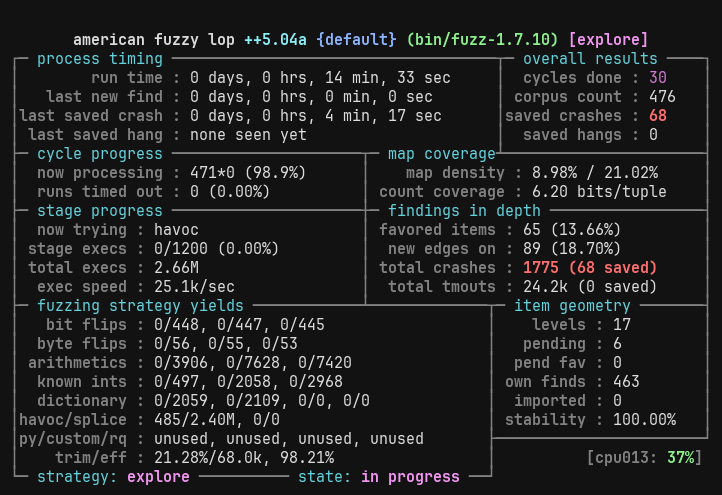
\includegraphics[width=0.49\textwidth]{afl-status-1.7.10.png}\hfill
  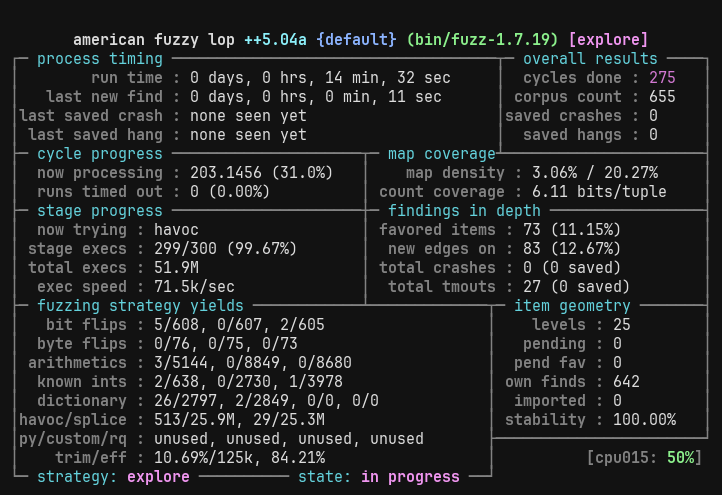
\includegraphics[width=0.49\textwidth]{afl-status-1.7.19.png}
  \caption{AFL++ status screens after 14.5~minutes: cJSON 1.7.10 (left), with 68 saved crashes, and cJSON 1.7.19 (right), with none.}
  \label{fig:aflstatus}
\end{figure*}

\begin{figure*}[!t]
  \centering
  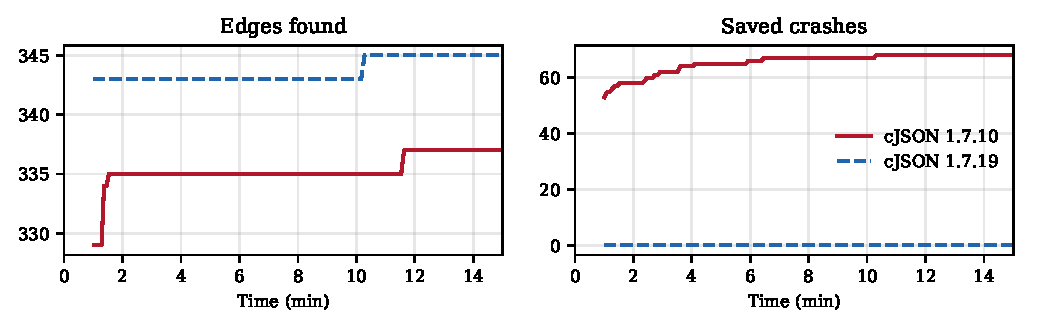
\includegraphics[width=0.85\textwidth]{afl-progress.pdf}
  \caption{Edges found and saved crashes over time for both releases (AFL++ writes the first sample after one minute).}
  \label{fig:aflprogress}
\end{figure*}

All 68 inputs crash the replay build of release 1.7.10 with the same
report: a heap-buffer-overflow, a read of one byte just past the copy of
the input, inside \texttt{cJSON\_Minify}. None of them crashes the replay
build of release 1.7.19. To find the root causes, a short script
follows the loop of \texttt{cJSON\_Minify} of release 1.7.10 and records
which branch first moves the read pointer past the terminating NUL.
Table~\ref{tab:findings} lists the three causes, each with the tail of
the input that \texttt{afl-tmin} minimised (\texttt{\textbackslash 0} is
the NUL byte). In every input, the parser accepts a valid value, such as
\texttt{0}, and ignores the bytes that follow it, because the harness
does not require termination. \texttt{cJSON\_Minify} then walks those
bytes and assumes that every string and comment is closed.

\begin{table*}[!t]
\caption{Findings of the AFL++ run on cJSON 1.7.10, grouped by root cause}
\label{tab:findings}
\centering
\scriptsize
\begin{tabularx}{\textwidth}{@{}L{0.4cm}L{3.3cm}cL{2.5cm}YL{1.4cm}L{1.9cm}L{1.2cm}@{}}
\toprule
\textbf{ID} & \textbf{Root cause} & \textbf{Inputs} & \textbf{Minimised tail} & \textbf{Sanitizer report} & \textbf{CWE} & \textbf{Known as} & \textbf{1.7.19} \\
\midrule
F1 & String literal not closed before the end of the input; the closing copy also copies the NUL and moves past it & 60 & \texttt{[0 ""00"\textbackslash 0} & heap-buffer-overflow, read of 1 byte, \texttt{cJSON.c:2642} (main loop); first after 0.7~s & CWE-125 & CVE-2019-11834 & No crash \\
F2 & Backslash as the last character of a string: the escape copy consumes the NUL & 2 & \texttt{"0000000\textbackslash\textbackslash 0} & heap-buffer-overflow, read of 1 byte, \texttt{cJSON.c:2682} (string loop); first after 2.9~s & CWE-125 & CVE-2019-11834 & No crash \\
F3 & Multiline comment \texttt{/*} not closed: the pointer skips two bytes past the NUL & 6 & \texttt{"00"/*0000000\textbackslash 0} & heap-buffer-overflow, read of 1 byte, \texttt{cJSON.c:2642} (main loop); first after 4.3~s & CWE-125 & CVE-2019-11835 & No crash \\
\bottomrule
\end{tabularx}
\end{table*}

An earlier run with the same settings, kept as a check, gave the same
picture: 63 crashes and one slow input on release 1.7.10, all from the
same three causes (the slow input is an F1 case that crashes at once on
the replay build), and no crash on release 1.7.19.

\subsection{Discussion}

The run found, within five seconds, the two faults that release 1.7.11
fixed, and \ac{ASan} turned reads that would otherwise go unnoticed into
crashes with an exact location. The faults sit behind a parser that
accepts a valid value followed by trailing bytes, while another function
reads those same bytes under different assumptions. In SecureBank~PT
the same gap would appear if the gateway and a banking service parsed a
request differently, which is what FZ-02 and FZ-03 test; the plan
therefore requires parsers that reject trailing data and native code
fuzzed under sanitizers (FZ-10). The run on release 1.7.19 shows only
that this harness and these seeds found nothing in 15~minutes, not that
the parser is free of faults. The run has further limits: one instance
per release, one harness, coverage measured only as AFL++ edges, and a
target that is a component like those of SecureBank~PT rather than part
of it. As expected from a fuzzer, it found memory faults and nothing
about authorisation, which the penetration test covers.
